\section{Graphische Programmierung}

\subsection{Definition von Graphischen Objekten}
Graphische Objekte bestehen letztendlich aus Punkten, die mit Kanten zu Dreiecken verbunden sind.\\
Man könnte auch denken, wieso denn nicht 4- oder 5-Ecke?\\
Jedes n-Eck, wobei 3 $\leq$ n, kann durch hinzufügen zusätzlicher Kanten nur mit Dreiecken dargestellt werden. Dreiecke haben zusätzlich den Vorteil, dass die eine Ebene im 3-dimensionalen kartesischen Koordinatensystem definieren. Dadurch kann das Dreieck als klarer Ebenenteil gezeichnet werden, wohingegen z.B. Vierecke nicht unbedingt in einer Ebene liegen und dadurch beim Zeichnen eventuell ohnehin als 2 getrennte Dreiecke gezeichnet werden müssten.\\

\subsection{Koordinatensysteme}
Wir betrachten das 3 dimensionale kartesische Koordinatensystem, welches als 3-dimensionales Orthogonalsystem definiert ist. Das bedeutet, dass es 3 Achsen gibt, die aus Vektoren bestehen, die paarweise Orthogonal zu sich stehen.\\
Wir unterscheiden weiter zwischen einem rechthändigen und linkshändigen Koordinatensystem, welche sich durch die Richtung der positiven z-Achse unterscheiden. Beim Rechtshändigen Koordinatensystem läuft die positive z-Achse zum betrachter hin, beim linkshändigen Koordinatensystem dementsprechend vom betrachter weg.
\\\\

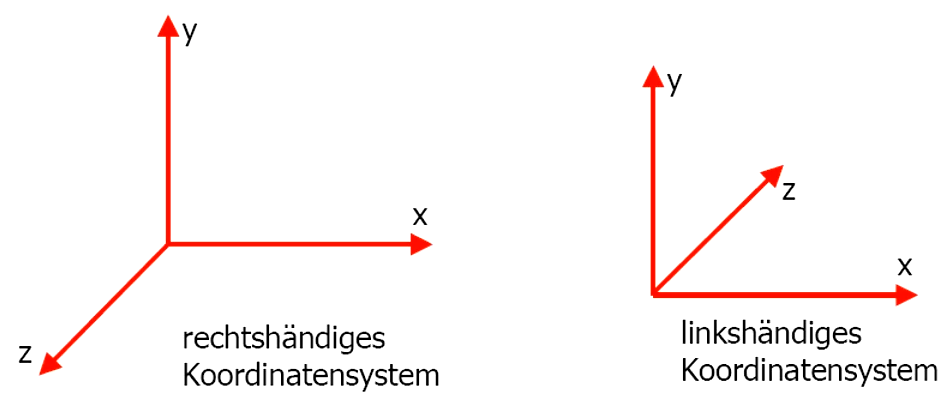
\includegraphics[width=400px]{images/Koordinatensysteme.png}

\subsection{Graphische Primitive in OpenGL}
In OpenGL können verschiedene \textit{Primitive} erzeugt werden. Das sind einfache Objekte, die von OpenGL auf Basis einzelner Punkte erzeugt werden. Diese kann man dann zusammenschließen, um komplexere Objekte zu erzeugen. Beispiele für Primitive sind hier gezeigt:

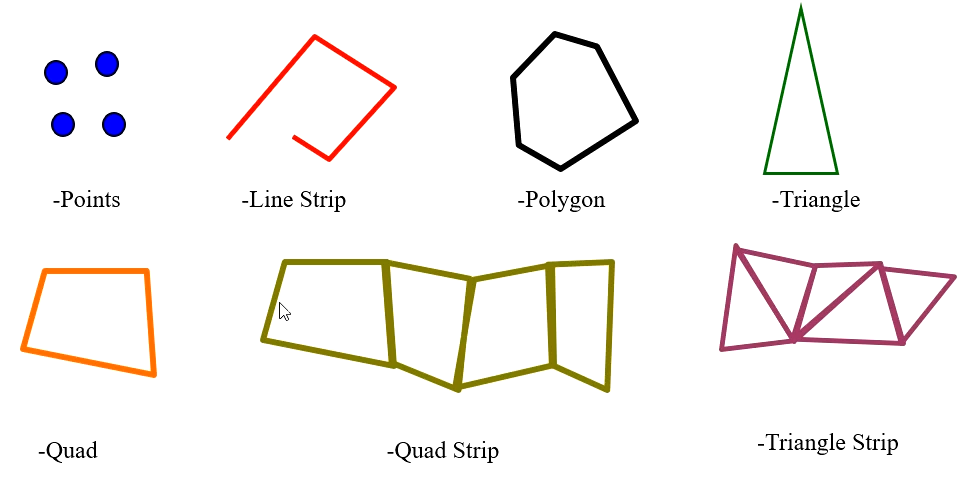
\includegraphics[width=400px]{images/openGlPrimitives.png}

\subsection{Transformationen Graphischer Objekte}
Jedes Objekt kann zunächst irgendwo in seinem Koordinatensystem definiert werden. Diese Platzierung nennt man nun die Platzierung in seinem \textit{lokalen Koordinatensystem}.\\
Durch verschiedene Transformationen kann das Objekt verändert werden, um seine Position, Ausrichtung und Größe zu verändern und schließlich im \textit{Weltkoordinatensystem} platziert werden.\\
Somit können Objekte einmalig durch geeignete Funktionen definiert werden und dann durch Transformationen für ihre aktuelle Verwendung angepasst werden. Die Transformationen sind konkret:
\begin{itemize}
    \item \textbf{Translation:} Verschiebung der Koordinaten eines Punktes. Dies entspricht der Addition eines Verschiebungsvektors auf den Ortsvektor des Punktes.
    \item \textbf{Rotation:} Drehen des Punktes um eine Koordinatenachse. Hierbei ist der Winkel entgegen des Uhrzeigersinns zu lesen.
    \item \textbf{Skalierung:} Multiplikation des Ortsvektors eines Punktes mit einem Skalar. Wird diese Operation für alle Punkte eines Objektes vorgenommen entsteht eine Stauchung oder Streckung entlang der Koordinatenachsen.
\end{itemize}

\subsection{Szenegraph}
Ein Szenegraph ist eine Datenstruktur, die eingesetzt werden kann, um mehrereg graphische Objekte zu einer Szene zusammenzuschließen.\\
Der Szenegraph ist ein gerichteter Zyklenfreier Graph. Das bedeutet, dass im Gegensatz zu einem Baum, ein Kindknoten auch mehrere Elternknoten haben kann, jedoch die Richtung der Abhängigkeiten einheitlich von Wurzel zu Blättern verläuft:
\\\\

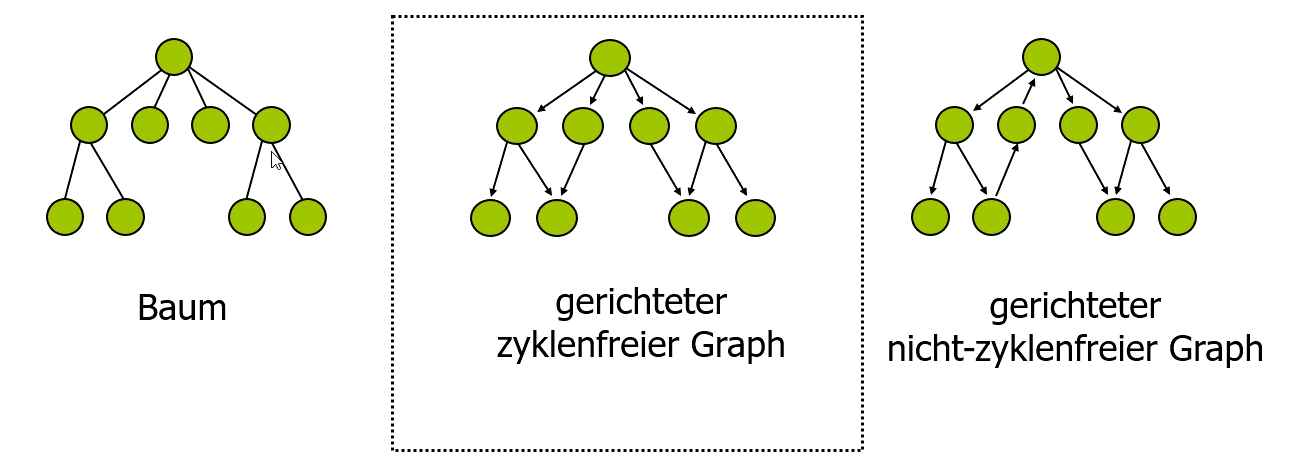
\includegraphics[width=400px]{images/gerichteterZyklenfreierGraph.png}

Die Knoten des Szenegraphen können Entweder Gruppen, Geometrien oder Transformationen sein:
\\

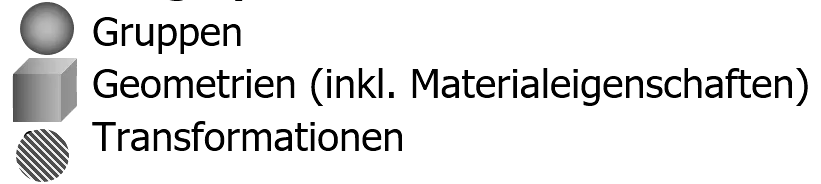
\includegraphics[height=50px]{images/Szenegraph_Knotentypen.png}
\\\\\\
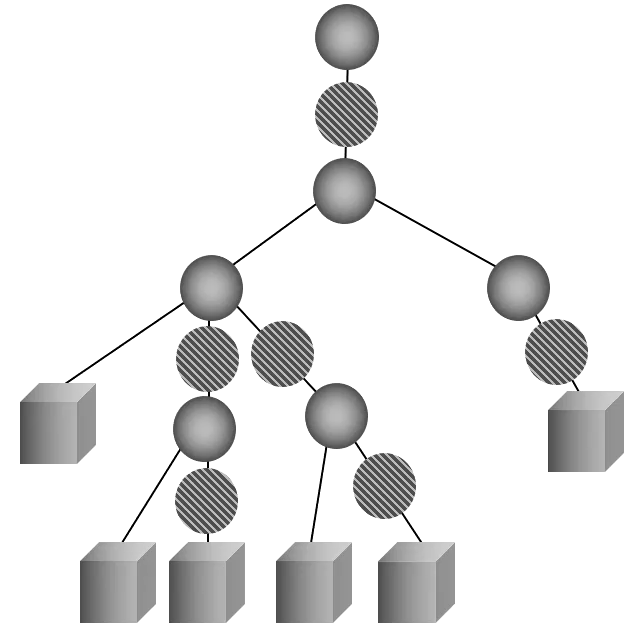
\includegraphics[width=200px]{images/Szenegraph_Beispiel.png}
\\\\

\textbf{Gruppen} bezeichnen hierbei zusammenfassungen von Punkten, die Graphische Objekte bilden. Transformationen beziehen sich dann auf alle Objekte, die im Szenegraphen unter ihnen liegen.\\
Dadurch kann man die Zusammenhänge komplexerer Objekte geeignet darstellen. Zum Beispiel soll eine Komplexe Figur, z.B. ein Mensch, sich generell im Raum bewegen können (Translation). Diese Translation wirkt sich dann auf alle Gruppen, die den Mensch bilden aus (als z.B. seinen Kopf, Rumpf, Arme und Beine). Der Mensch kann aber auch den Arm heben. Diese Translation soll sich dann also nur auf den Arm der Figur auswirken. Läuft der Mensch aber und hebt dabei seine Hand, so muss auf dem Arm offensichtlich sowohl die Translation des Körpers als auch die des Arms angewendet werden. So sieht man, dass der Arm im Szenegraphen also eine Gruppe sein muss, deren Eltengraphen die gesamte Figur "Mensch" ist.

\subsection{Arbeiten mit OpenGL}
OpenGL ist im Grunde eine Art Zustandsautomat und sehr explizit. Zunächst sind keine Einstellungen vorgenommen. Wird durch einen Funktionsaufruf eine Einstellung (z.B. der Farbe) Vorgenommen, so wird sie so lange beibehalten, bis sie geändert wird.\\
Ein weiteres Beispiel ist, dass der Bildschirm jedes Frame explizit gecleared werden muss, falls das vorherige Bild verworfen werden soll. Denn das vorherige Bild würde bestehen bleiben und nur die Stellen an denen Objekte gerendert werden aktualisiert werden.\\

\subsubsection*{Wie berechnet OpenGL Transformationen?}
Transformationen von Vektoren können mathematisch generell durchgeführt werden, indem eine Transformationsmatrix definiert wird, die mit dem Vektor multipliziert wird und so einen neuen Vektor ergibt. Sollen mehrere Transformationen auf einen Punkt angewendet werden, so muss ein Vektor also nacheinander mit mehreren Matrizen multipliziert werden. Dabei ist zu beachten, dass die Multiplikation von Matrizen nicht kommutativ aber assoziativ ist.\\

\[
    \begin{pmatrix}
        a & b & c \\
        d & e & f \\
        g & h & i
    \end{pmatrix}
    \cdot
    \left(
    \begin{pmatrix}
            a & b & c \\
            d & e & f \\
            g & h & i
        \end{pmatrix}
    \cdot
    \begin{pmatrix}
            a \\
            d \\
            g
        \end{pmatrix}
    \right)
    =
    \left(
    \begin{pmatrix}
            a & b & c \\
            d & e & f \\
            g & h & i
        \end{pmatrix}
    \cdot
    \begin{pmatrix}
            a & b & c \\
            d & e & f \\
            g & h & i
        \end{pmatrix}
    \right)
    \cdot
    \begin{pmatrix}
        a \\
        d \\
        g
    \end{pmatrix}
\]
\\

OpenGL geht so vor, dass es immer, wenn eine Transformation definiert wird, diese mit der aktuellen globalen Tranformationsmatrix multipliziert (Zu Beginn ist diese Matrix die Dreidimensionale Einheitmatrix). Immer wenn dann ein Objekt definiert wird, wird diese aktuelle Transformationsmatrix auf das Objekt angewendet.\\
Weil die Multiplikation assoziativ ist, entspricht das Ergebnis der Multiplikation in jedem Fall dem Ergebnis, das entsteht, wenn man den Vektor von rechts nach links mit den Matrizen multipliziert. Will man also eine bestimmte Transformation vor einer anderen durchführen, so muss sie weiter rechts stehen, um früher angewendet zu werden.
\subsubsection*{Matrizenstack}
Neben der aktuellen Transformationsmatrix, die sich immer auf die aktuell definierten Objekte bezieht, speichert OpenGL auch noch einen sogenannten Matrizenstack.\\
Ein Aufruf von \textit{glPushMatrix()} legt die aktuelle Transformationsmatrix auf dem Stack ab. Die Matrix wird aber auch als aktuelle Matrix weiter verwendet.\\
Ein Aufruf von \textit{glPopMatrix()} ersetzt die aktuelle Transformationsmatrix durch die zuletzt gepushte Matrix und entfernt sie vom Matrizenstack.\\
Somit kann also eine Matrix gesichert und später wiederverwendet werden, wie etwa bei Unterprogrammaufrufen in ASM, wenn man zunächst die aktuellen Register auf dem Stack rettet.\\
Zum Beispiel könnte man sich vorstellen, dass ein um 45 Grad gedrehter Würfel erzeugt werden soll, der außerdem um 2 Längen entlang der negativen y-Achse verschoben ist und ein Würfel im Ursprung des Koordinatensystem gezeichnet werden soll. Wenn man nicht den Matrizenstack nutzt würde das in etwa so aussehen:
\begin{itemize}
    \item glRotatef(45, 1.0, 0.0, 0.0);
    \item glTranslatef(0.0, -2.0, 0.0);
    \item Cube();
    \item glRotatef(-45, 1.0, 0.0, 0.0);
    \item glTranslatef(0.0, 2.0, 0.0);
    \item Cube();
\end{itemize}
Mit Benutzung des Matrizenstacks ist das Wiederherstellend er ursprünglichen Transformationsmatrix einfacher:
\begin{itemize}
    \item glPushMatrix();
    \item glRotatef(45, 1.0, 0.0, 0.0);
    \item glTranslatef(0.0, -2.0, 0.0);
    \item Cube();
    \item glPopMatrix();
    \item Cube();
\end{itemize}

\subsubsection*{Definition von Dreiecksstreifen}
Wenn komplexe Objekte aus Dreiecken gebildet werden sollen, dann sind viele Eckpunkte eines vorherigen Dreiecks wieder ein Eckpunkt eines folgenden Dreiecks und damit die definition und Speicherung dieses redundant. Somit kann durch das Benutzen von  \textit{GL\_TRIANGLE\_STRIP}s effizienter vorgegangen werden.\\

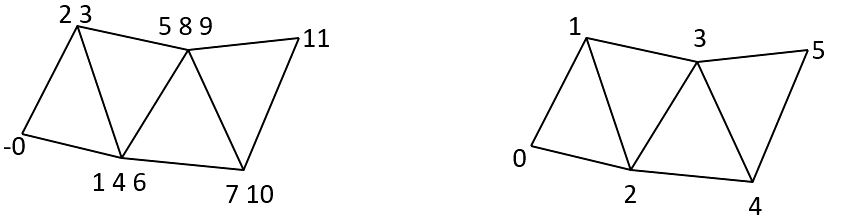
\includegraphics[width=350px]{images/glTriangleStrip.png}

\subsubsection*{Definition von Farben und Texturen}
Farben und Texturen werden jeweils global umgestellt und gelten dann für alle folgenden Punkte (siehe Zustandsautomat). Flächen oder Linien, die letztendlich durch die Verbindung von Punkten entstehen erhalten dann die lineare Interpolation der Farb und Texturwerte der zugehörigen Punkte:\\

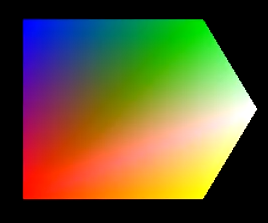
\includegraphics[height=80px]{images/openGlColors.png}

\subsubsection*{Rotation von Objekten um sich selbst}
Soll ein Objekt um seinen eigenen Mittelpunkt gedreht werden, so kann dieses Objekt zunächst in den Ursprung des Koordinatensystems bewegt werden, dann die Rotation durchgeführt werden und dann muss es wieder an seinen ursprünglichen Platz zurückbewegt werden.\\
Auf diese Weise kann der Standort des Objektes vor der Rotation erhalten bleiben.\\
Hierbei ist auch zu beachten, dass die Rücktranslation zuerst angegeben werden muss, dann die Rotation und dann die Translation, da wie gesagt die zuletzt angegebene Transformation zuerst angewendet wird.